\documentclass[dvips,10pt]{article}
\usepackage{graphicx}
\setlength{\oddsidemargin}{-0.3in}
\setlength{\textwidth}{7.0in}
\setlength{\topmargin}{-0.70in}
\setlength{\textheight}{9.5in}
\pagestyle{myheadings}
\markright{ {\rm {
Quarterly OPEN AE/SAE Report
 \hspace{2em}
Thu Feb 05 15:37:01 EST 2009
\hfill
\hspace{3em}
}}}
\headsep=0.2in
\begin{document}
\vspace*{1in}
\begin{center}
{\Huge{CONFIDENTIAL}}
\end{center}
\vspace*{0.5in}
\begin{center}
{\Huge{GLND}}
\end{center}
\vspace*{0.25in}
\begin{center}
{\Huge{
Quarterly OPEN AE/SAE Report
}}
\end{center}
\begin{center}
{\Huge{
 
}}
\end{center}
\begin{center}
{\Huge{Atlanta, GA}}
\end{center}
\vspace*{1in}
\begin{center}
\noindent
{\Large{Includes patients enrolled and follow-up data received as of Thu Feb 05 15:37:01 EST 2009}}
\end{center}
\vspace*{0.5in}
\begin{center}
{\Large{Report prepared  Thu Feb 05 15:37:01 EST 2009 }}
\end{center}
\clearpage
\vspace*{1in}
\begin{center}
{\Huge{Table of Contents}}
\end{center}
\listoftables
\listoffigures
\clearpage
\begin{table}[t]
\caption
{ AE Unrelated to Glutamine. }
\begin{center}
\begin{tabular}{ @{}l@{}
@{}l@{}@{}p{1.5em}@{}@{}c@{}
}
\hline

& \parbox{6em}{\begin{center}Adverse Event\end{center}} && \parbox{6em}{\begin{center}Total n=80\end{center}} \\

\hline

\\
& Respiratory distress && 17( 15) 18.8\% \\
& Tracheostomy && 16( 16) 20.0\% \\
& Significant pulmunary aspiration && 0(  0)  0.0\% \\
& Pneumothorax && 1(  1)  1.3\% \\
& Pulmonary emboli && 1(  1)  1.3\% \\
& Wound dehiscence && 2(  2)  2.5\% \\
& New onset significant hemorrhage && 11(  8) 10.0\% \\
& 
Mechanical intestinal obstr. && 1(  1)  1.3\% \\
& Myocardial infarction && 2(  1)  1.3\% \\
& Cerebrovascular accident && 4(  4)  5.0\% \\
& Re-admission to ICU/SICU && 9(  9) 11.3\% \\
& New onset significant skin rash && 1(  1)  1.3\% \\
& 
Non-infectious pancreatitis && 0(  0)  0.0\% \\
\\
\hline \\

\end{tabular}


\parbox{ 5in }{ \# AEs (\# Pat) \% Pat } \\
 \vspace{1em}\end{center}
 \end{table}
\begin{table}[t]
\caption
{ AE Potentially Related to Glutamine. }
\begin{center}
\begin{tabular}{ @{}l@{}
@{}l@{}@{}p{1.5em}@{}@{}c@{}
}
\hline

& \parbox{6em}{\begin{center}Adverse Event\end{center}} && \parbox{6em}{\begin{center}Total n=80\end{center}} \\

\hline

\\
& Worsening renal function && 6(  6)  7.5\% \\
& Worsening hepatic function && 2(  2)  2.5\% \\
& Encephalopathy && 2(  2)  2.5\% \\
& Hyperglycemia && 65( 30) 37.5\% \\
& Hypoglycemia && 12(7/35) 20.0 \\
\\
\hline \\

\end{tabular}


\parbox{ 5in }{ \# AEs (\# Pat) \% Pat \newline Hypoglycemia information collected since April 1,2008 only } \\
 \vspace{1em}\end{center}
 \end{table}
\clearpage
\begin{table}[t]
\caption
{ SAE. }
\begin{center}
\begin{tabular}{ @{}l@{}
@{}l@{}@{}p{1.5em}@{}@{}c@{}
}
\hline

& \parbox{6em}{\begin{center}Adverse Event\end{center}} && \parbox{6em}{\begin{center}Total n=80\end{center}} \\

\hline

\\
& Death && 15( 15) 18.8\% \\
& Anaphylactic reaction && 0(  0)  0.0\% \\
& Seizure && 1(  1)  1.3\% \\
& Cardiopulmonary arrest && 3(  3)  3.8\% \\
& Re-hospitalization w/in 30 days && 18( 16) 20.0\% \\
& Re-operation w/in 30 days && 30( 15) 18.8\% \\
& New cancer diagnosis && 0(  0)  0.0\% \\
& Congenital anomaly/disorder && 0(  0)  0.0\% \\
\\
\hline \\

\end{tabular}


\parbox{ 5in }{ \# AEs (\# Pat) \% Pat \newline Per protocol, an SAE form is completed only for events that occur within 30
  days of study drug discontinuation. } \\
 \vspace{1em}\end{center}
 \end{table}
\begin{table}[t]
\caption
{ Mortality Rates by Center. }
\begin{center}
\begin{tabular}{ @{}l@{}
@{}l@{}@{}p{1.5em}@{}@{}c@{}@{}p{1.5em}@{}@{}c@{}@{}p{1.5em}@{}@{}c@{}@{}p{1.5em}@{}@{}c@{}@{}p{1.5em}@{}@{}c@{}
}
\hline

& \parbox{6em}{\begin{center}Period\end{center}} && \parbox{6em}{\begin{center}Overall\end{center}} && \parbox{6em}{\begin{center}Emory\end{center}} && \parbox{6em}{\begin{center}Miriam\end{center}} && \parbox{6em}{\begin{center}Vanderbilt\end{center}} && \parbox{6em}{\begin{center}Colorado\end{center}} \\

\hline

\\
& 6-month && 22/79 (27.8\%) && 9/33 (27.3\%) && 3/9 (33.3\%) && 6/19 (31.6\%) && 4/18 (22.2\%) \\
& In-hospital && 11/79 (13.9\%) && 5/33 (15.2\%) && 2/9 (22.2\%) && 4/19 (21.1\%) && 0/18 (0.0\%) \\
& 28-Day && 11/79 (13.9\%) && 5/33 (15.2\%) && 3/9 (33.3\%) && 3/19 (15.8\%) && 0/18 (0.0\%) \\
\\
\hline \\

\end{tabular}

\end{center}
 \end{table}
\clearpage

\begin{figure}
\resizebox{6.8in}{!}{\rotatebox{0}{\includegraphics{deathdetails.ps}}}
\end{figure}
\clearpage

\begin{figure}
\resizebox{6.8in}{!}{\rotatebox{0}{\includegraphics{deathdetails1.ps}}}
\end{figure}
\clearpage
\end{document}
